\documentclass[12pt]{article}
\usepackage{sammath}

\newcommand{\unc}{\texttt{uncertainty}~$\ang{(a)(a)}-\ang{(a)}\ang{(a)}$}
\newcommand{\tem}{\texttt{temerity}~$2\ang{(a)}(\ang{(ab)(b)}-\ang{(ab)}\ang{(b)})$}
\newcommand{\per}{\texttt{peril}~$\ang{(ab)}(\ang{(a)(b)}-\ang{(a)}\ang{(b)})$}

\begin{document}
    \customtitle{Perturbative Analysis of SGD}
    %\customsubtitle{Dan Roberts (\texttt{roberts@ias.edu}) and Samuel Tenka (\texttt{coli@mit.edu})}

    \customsection{Datatype of the Loss Landscape}
    \customsection{Coefficients of Generalization}
        Let
        $$
            INT = \ang{(a)}\ang{(a)}
        $$$$
            UNC = \ang{(a)(a)}-\ang{(a)}\ang{(a)}
        $$$$
            PAS = 2\ang{(a)}\ang{(ab)(b)}
        $$$$
            TEM = 2\ang{(a)}(\ang{(ab)(b)}-\ang{(ab)}\ang{(b)})
        $$$$
            PER = \ang{(ab)}(\ang{(a)(b)}-\ang{(a)}\ang{(b)})
        $$

        One finds:
        $$
            \expec L_{\text{SGD}}(\eta) =
                () + \eta {T \choose 1} INT +
                \eta^2 \wrap{
                    {T \choose 2} \wrap{\frac{PAS}{2} + \frac{PAS}{4}} + 
                    {T \choose 1} \wrap{\frac{PAS}{4} + \frac{PER}{2}}
                } + \cdots
        $$
        while:
        $$
            \expec L_{\text{GD}}(\eta) =
                () + \eta {T \choose 1} INT  +
                \eta^2 \wrap{
                    {T \choose 2} \wrap{\frac{PAS}{2} + \frac{TEM}{2N} + \frac{PAS}{4} + \frac{PER}{2N}} + 
                    {T \choose 1} \wrap{\frac{PAS}{4} + \frac{PER}{2N}}
                } + \cdots
        $$

    \customsection{Toy Examples}
        \customsubsection{Shifting Valleys}
            Let $L(x, (A, B)) = A + (B - Ax)^2 - A^2$, where the data samples $x\in \RR^1$ obey a standard normal law.   
            The weights $(A, B)\in \RR^2$ we initialize to $(1, 1)$.
            The expected loss is $\expec L(A, B) = A + B^2$. 

            \begin{figure}[h]
                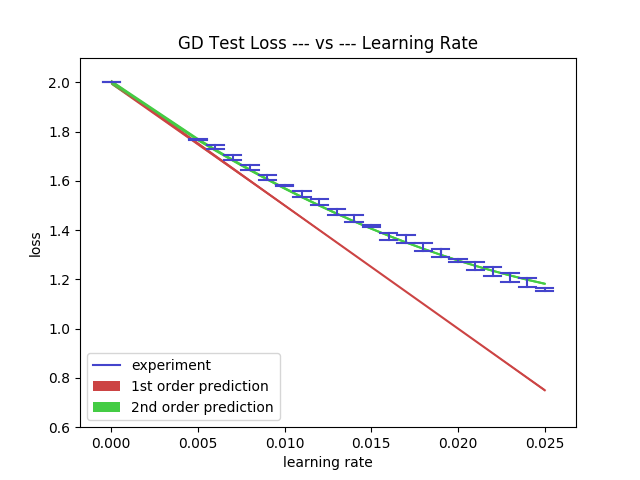
\includegraphics[width=8cm]{imgs/gauss.10/out-gd}
                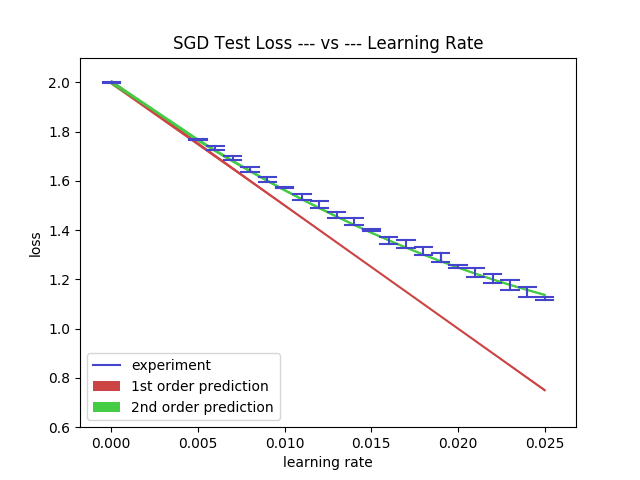
\includegraphics[width=8cm]{imgs/gauss.10/out-sgd}
                \caption*{
                    {\bf Above}: for the Valley Task, our $2$nd order corrections for test-time loss match experiment
                    (for $T=10$ and $\eta \leq 0.025$; $\eta$ of this magnitude suffice to halve the test loss).
                }
            \end{figure}
            \begin{figure}[h]
                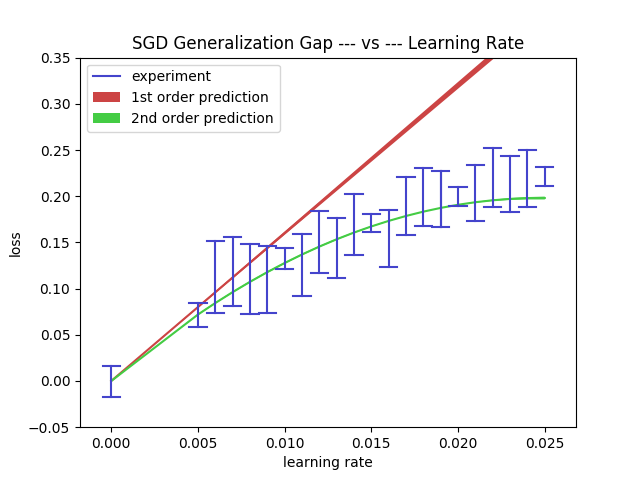
\includegraphics[width=8cm]{imgs/gauss.10/gen-sgd}
                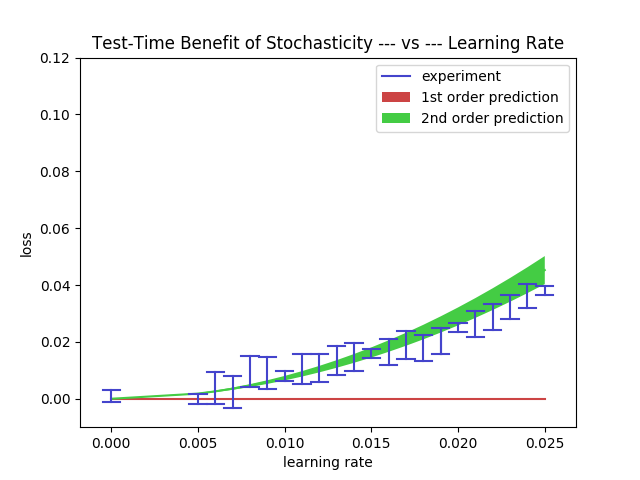
\includegraphics[width=8cm]{imgs/gauss.10/out-diff}
                \caption*{
                    {\bf Above}: for the Valley Task, experiments verify
                        ({\bf left})  the predicted dependence of generalization gap on \unc~ and
                        ({\bf right}) the resulting dependence of SGD's test-time outperformance of GD on \tem~ and \per.  
                }
            \end{figure}


        \customsubsection{Valley of Death}
            Let $L(x, (A, B)) = A + (B - Ax)^4 - 3A^4$, where the data samples $x\in \RR^1$ obey a standard normal law.   
            The weights $(A, B)\in \RR^2$ we initialize to $(1, 1)$.
            The expected loss is $\expec L(A, B) = A + 2A^2 B^2 + B^4$. 




\end{document}
